\subsection{Analysis of UK weather station data}\label{subsec-data-2} 

\begin{figure}[t]
\centering
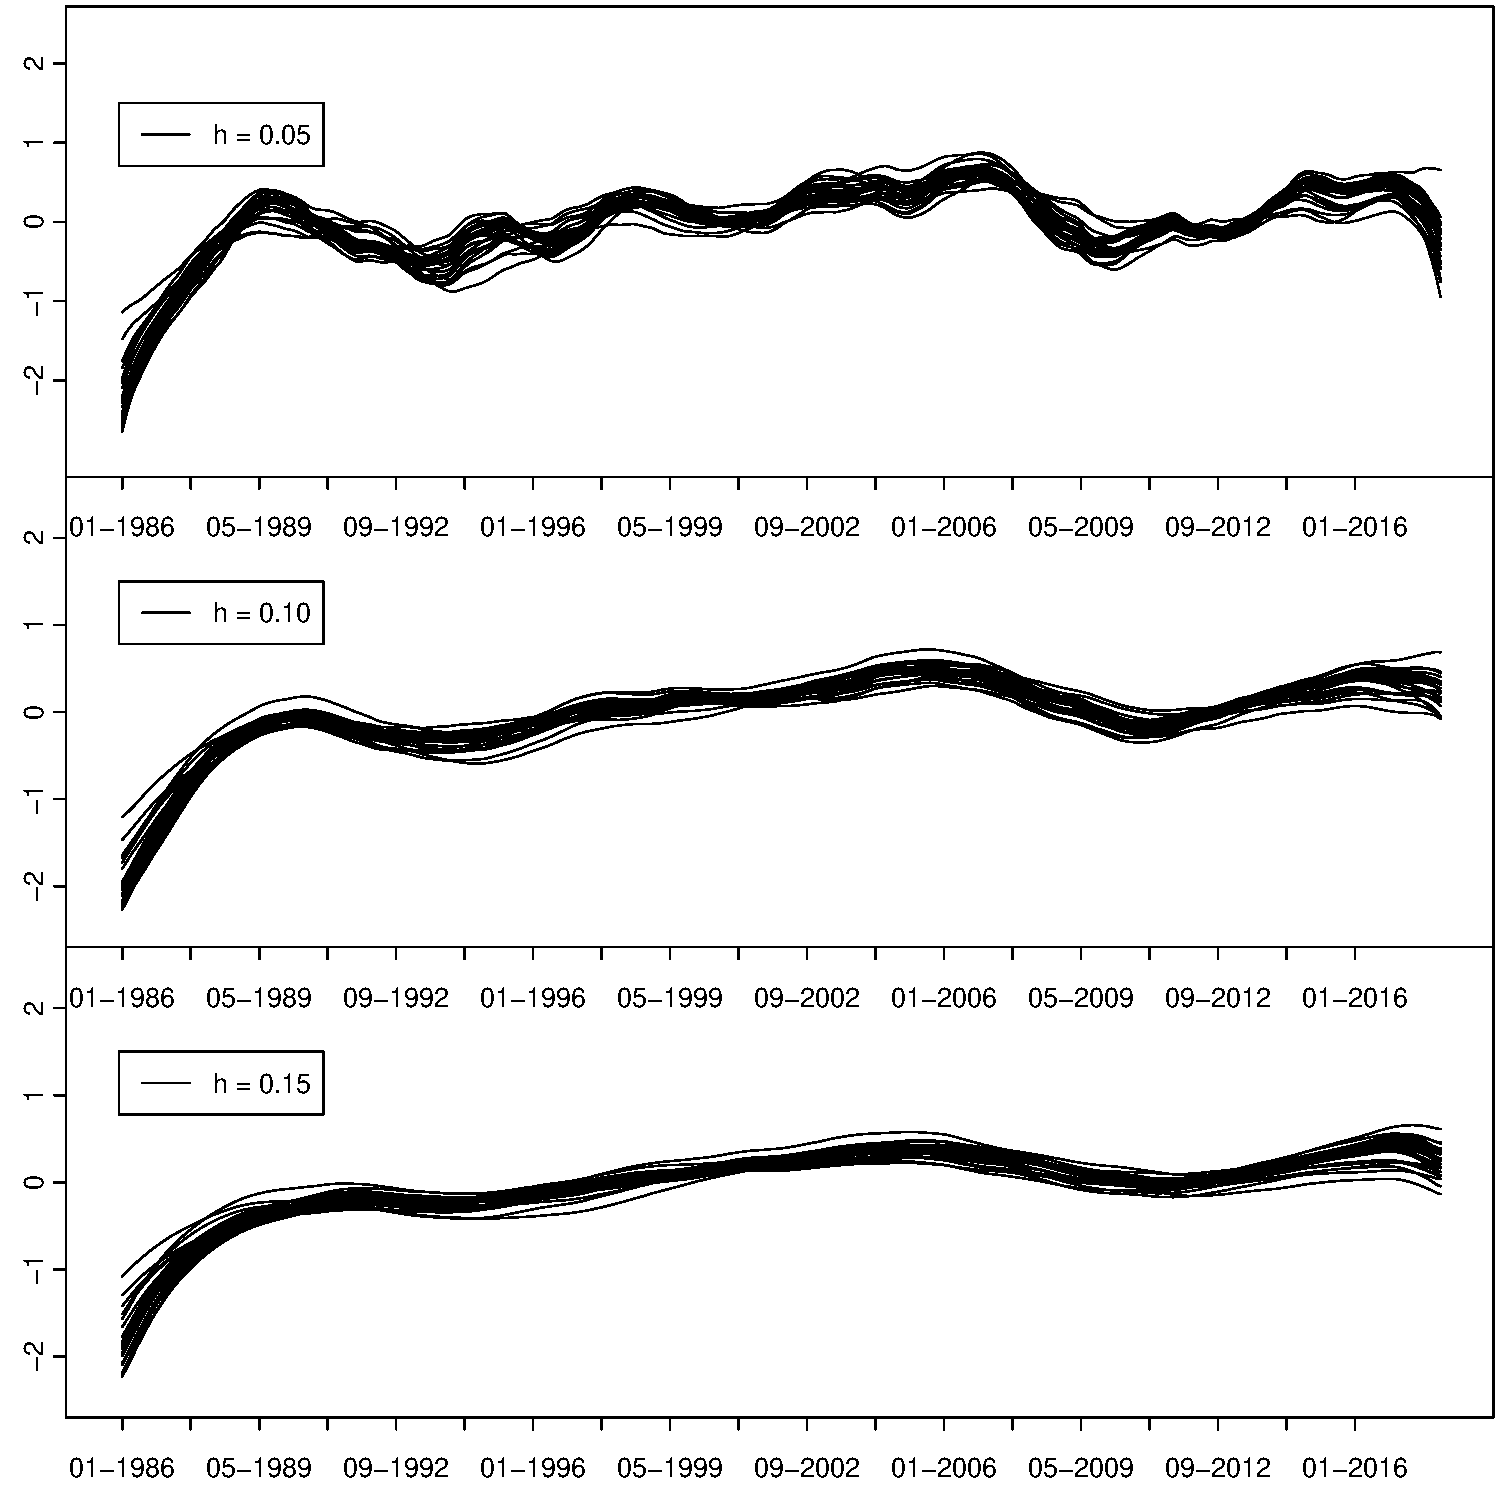
\includegraphics[width=0.8\textwidth]{Plots/stations_data.pdf}
\vspace{0.2cm}
\caption{Local linear kernel estimates of the $n=25$ time trends from the application of Section \ref{subsec-data-2}. Each panel shows the estimates for a different bandwidth $h$.}\label{plot-results-app2}
\end{figure}


To illustrate our test method from Section \ref{sec-test-equality}, we examine a dataset of monthly mean temperatures from $34$ different UK weather stations. The data are publicly available on the webpage of the UK Met Office. We use a subset of $25$ stations for which data are available over the time span from $1986$ to $2017$. We thus observe a time series $\mathcal{Y}_i = \{Y_{it}: 1 \le t \le T \}$ of length $T = 386$ for each station $i \in \{1,\ldots,25\}$. The time series $\mathcal{Y}_i$ is assumed to follow the model 
\begin{equation}\label{model2-app}
Y_{it} = \alpha_i(t) + m_i\Big(\frac{t}{T}\Big) + \varepsilon_{it}, 
\end{equation}
where $m_i$ is an unknown nonparametric time trend and $\alpha_i(t)$ is a month-specific intercept which captures the seasonality pattern in the data. We suppose that $\alpha_i(t) = \alpha_i(t + 12 \ell)$ for any integer $\ell$, that is, we have a different intercept $\alpha_i(k)$ for each month $k = 1,\ldots,12$. The test method and the underlying theory from Section \ref{sec-test-equality} can be easily adapted to model \eqref{model2-app}, which is a slight extension of model \eqref{model2}. The details are provided below. As in Section \ref{subsec-data-1}, the error process $\mathcal{E}_i = \{ \varepsilon_{it}: 1 \le t \le T \}$ is assumed to have the AR(1) structure $\varepsilon_{it} = a_i \varepsilon_{i,t-1} + \eta_{it}$ for each $i$, where $\eta_{it}$ are i.i.d.\ innovations with mean zero.  



